%%%%%%%%%%%%%%%%%%%%%%%%%%%%%%%%%%%%%%%%%%%%%%%%%%%%%%%%%%%%%%%%%%%%%%%%%%%%%%%%%%%%%%%%%%%%%%%%%%%%%
%
%   Version     : 2.0
%
%   Filename    : main.tex
%
%   Description : This is the main file for the LaTeX thesis proposal document template.
%                 The template is intended for use by BSCS students. 
%
%                It is assumed that you can learn how to use LaTeX on your own.
%                Please check/read the following online LaTeX book:
%
%                                 http://en.wikibooks.org/wiki/LaTeX
%     
%   Author      : Florante R. Salvador
%
%   Contributors: 1.  Karlo Campos 
%                     a. margin settings for DLSU thesis paper 
%   
%   Notes       : Please email florante.salvador@dlsu.edu.ph for comments, suggestions, ideas etc.
%
%   Reference:
%
%
%   History/Updates:
%      March 12, 2009 -- created version 1.0 for release to CSC701M (Methods of Research) students
%      May 30, 2009   -- updated Title page and Abstract for undergrad ST students
%
%      Feb 27, 2015 -- Created Version 2 (major overhaul): changed class to report, created a figures folder, 
%                               removed unnecessary packages, added new comments  based on Ethel Ong's slides
%
%%%%%%%%%%%%%%%%%%%%%%%%%%%%%%%%%%%%%%%%%%%%%%%%%%%%%%%%%%%%%%%%%%%%%%%%%%%%%%%%%%%%%%%%%%%%%%%%%%%%%%

%%%%%%%%%%%%%%%%%%%%%%%%%%%%%%%%%%%%%%%%%%%%%%%%%%%%%%%%%%%%%%%%%%%%%%%%%%%%%%%%%%%%%%%%%%%%%%%%%%%%%%%%%%%%%%%%%%%%%%%
%
%  Filename   : preamble.tex
%
%  Description: Preamble file to :
%               a. specify related packages
%               b. set margins, commands, etc.
%
%  Note       : Edit the margin settings for your own printer
%                  You may add your own commands, environments (it is assumed that you know what you're doing.)
%
%%%%%%%%%%%%%%%%%%%%%%%%%%%%%%%%%%%%%%%%%%%%%%%%%%%%%%%%%%%%%%%%%%%%%%%%%%%%%%%%%%%%%%%%%%%%%%%%%%%%%%%%%%%%%%%%%%%%%%%

%\documentclass[12pt,titlepage,onepage, letterpaper]{article}

\documentclass[12pt,titlepage,onepage, letterpaper]{report}


%
%-- specify related packages
%

%
% \usepackage[utf8x]{inputenc}
%

\usepackage{apacite}           %-- APA style citation 
                               %-- refer to http://www.ctan.org/tex-archive/biblio/bibtex/contrib/apacite/

%
%  \usepackage{ucs}
%


\usepackage{amsmath}           %-- American Math Society packages
\usepackage{amsfonts}
\usepackage{amssymb}


\usepackage{graphicx}          %-- graphicx package needed for including figures in JPG or PNG format
 
%
%\usepackage{graphics}          %-- graphics related package (this was commented out) use when image is in EPS format
%
\usepackage{longtable}
\usepackage{lscape}
\usepackage{tabu}
\usepackage{verbatim}          %-- this package allows you to have multiple lines of comments by
                               %-- example:
                               %   \begin{comment}
                               %        ...your text here...
                               %   \end{comment}  

\usepackage{color}             %-- allows use of color with text
                               %-- example:  \textcolor{red}{This is the colored text in red.}
\usepackage{graphicx}
\usepackage{url}  %-- allows use of URLs example: \url{https:\ccs1.dlsu.edu.ph}


%
%-- set margins,  you may need to edit this for your own printer
%
\topmargin 0.0in
\oddsidemargin 0.0in
\evensidemargin 0.0in

\voffset 0.0in
\hoffset 0.5625in

\textwidth 5.75in
\textheight 8.5in


\parskip 1em
\parindent 0.25in

\bibliographystyle{apacite}            %-- use APA citation scheme

\hyphenation{ana-lysis know-ledge}     %-- LaTeX may not hyphenate correctly some words you use in your document
                                       %-- use \hyphenation to instruct LaTeX how to do it correctly, example above

\newcommand{\degree}{^{\circ}}         %-- use \newcommand to create your own "commands"
                                       %-- \newcommand works like the #define you learned in your COMPRO1 class

\newcommand{\etal}{et al.}


%\newcommand{\sinag}{\emph{Sinag}}
%\newcommand{\sinagtwo}{\emph{Sinag2}}

\newcommand{\figref}[1]{Figure \ref{#1}}
\newcommand{\appref}[1]{Appendix \ref{#1}}

%-- \newcommand{\Section}[1]{\section{#1}\setcounter{figure}{0}\setcounter{table}{0}}

%\newcommand{\shade}{\multicolumn{1}{|>{\columncolor[gray]{0.25}}c|}{}}
%\newcommand{\tableheader}[1]{\rowcolor{black}\color{white}{#1}}
%\newcommand{\cell}[2]{\multicolumn{1}{#1}{#2}}
%\newcommand{\definition}[2]{\textbf{\textit{#1}} --- #2}
%\newcommand{\itembit}[1]{\item \textbf{\textit{#1}}}
%\newcommand{\sgdef}[2]{\parbox[t][][t]{1.75in}{\textbf{#1}} \> \parbox[t][][t]{4.0in}{#2}\\\\}

%\newenvironment{sinagglossary}{\begin{flushleft}
%\begin{tabbing}
%\hspace{1.75in}\=\\}{\end{tabbing}\end{flushleft}}

\newcommand{\thestitle}[1]{{\Large \textsc{#1}}}


%---
%  \renewcommand{\thefigure}{\thesection.\arabic{figure}}
%  \renewcommand{\thetable}{\thesection.\arabic{table}}
%  \renewcommand{\contentsname}{Table of Contents}




                %-- includes LaTeX source file for the preamble 
                                  %-- include packages, sets the margin sequence, and many more... 
                                  %-- your job: check if the settings are suitable for your own printer

\graphicspath{{figures/}}  %-- figures is the name of the folder containing images JPG or PN

\begin{document}

%%%%%%%%%%%%%%%%%%%%%%%%%%%%%%%%%%%%%%%%%%%%%%%%%%%%%%%%%%%%%%%%%%%%%%%%%%%%%%%%%%%%%%%%%%%%%%%%%%%%%%
%
%   Filename    : title_page.tex 
%
%   Description : This file will contain your Title Page.
%                 
%%%%%%%%%%%%%%%%%%%%%%%%%%%%%%%%%%%%%%%%%%%%%%%%%%%%%%%%%%%%%%%%%%%%%%%%%%%%%%%%%%%%%%%%%%%%%%%%%%%%%%

\begin{titlepage}
\centering


%-- **EDIT** the following line to indicate your thesis title
\thestitle{Community Detection in Social Networks}

\vspace{1.75cm}
A Thesis Proposal\\
Presented to\\
the Faculty of the College of Computer Studies\\
De La Salle University Manila

\vspace{1.75cm}
In Partial Fulfillment\\
of the Requirements for the Degree of\\
Bachelor of  Science in Computer Science

\vspace{1.75cm}
by\\
%-- **EDIT** the following line to indicate your name 
\vspace{1cm}

FERNANDEZ, Ryan Austin \\
POBLETE, Clarisse Felicia M.  \\
SAN PEDRO, Marc Dominic  \\
TAN, Johansson E.  \\

\vspace{1.75cm}
%-- **EDIT** the following line to indicate your adviser's name 
Charibeth K. CHENG \\
Adviser

\vspace{1.75cm}
\today
\end{titlepage}
              %-- includes LaTeX source file for the Title Page 
                                  %-- your job: **EDIT THIS FILE ** to indicate your own title, name, and thesis adviser's name

\begin{comment}
%%%%%%%%%%%%%%%%%%%%%%%%%%%%%%%%%%%%%%%%%%%%%%%%%%%%%%%%%%%%%%%%%%%%%%%%%%%%%%%%%%%%%%%%%%%%%%%%%%%%%%
%
%   Filename    : abstract.tex 
%
%   Description : This file will contain your abstract.
%                 
%%%%%%%%%%%%%%%%%%%%%%%%%%%%%%%%%%%%%%%%%%%%%%%%%%%%%%%%%%%%%%%%%%%%%%%%%%%%%%%%%%%%%%%%%%%%%%%%%%%%%%

\begin{abstract}
From 150 to 200 words of short, direct and complete sentences, the abstract 
should be informative enough to serve as a substitute for reading the thesis document 
itself.  It states the rationale and the objectives of the research.  

In the final thesis document (i.e., the document you'll submit for your final thesis defense), the 
abstract should also contain a description of your research results, findings, 
and contribution(s).

%
%  Do not put citations or quotes in the abract.
%

Keywords can be found at \url{http://www.acm.org/about/class/class/2012?pageIndex=0}.  Click the 
link ``HTML'' in the paragraph that starts with ''The \textbf{full CCS classification tree}...''.

\begin{flushleft}
\begin{tabular}{lp{4.25in}}
\hspace{-0.5em}\textbf{Keywords:}\hspace{0.25em} & Keyword 1, keyword 2, keyword 3, keyword 4, etc.\\
\end{tabular}
\end{flushleft}
\end{abstract}
                %-- this is the Abstract page
                                  %-- your job: **EDIT THIS FILE** to indicate your own abstract

\pagenumbering{roman}             %-- this will number pages as i, ii, iii, etc...
\setcounter{page}{2}

\tableofcontents                  %-- this command is used to generate the Table of Contents


\newpage
\listoffigures                    %-- this command is used to generate List of Figures

\newpage                       
\listoftables                     %-- this command is used to generate List of Tables

\newpage
\end{comment}

\pagenumbering{arabic}            %-- this will number pages as 1, 2, 3, etc...
\setcounter{page}{1}              


%%%%%%%%%%%%%%%%%%%%%%%%%%%%%%%%%%%%%%%%%%%%%%%%%%%%%%%%%%%%%%%%%%%%%%%%%%%%%%%%%%%%%%%%%%%%%%%%%%%%%%
%
%   Filename    : chapter_1.tex 
%
%   Description : This file will contain your Research Description.
%                 
%%%%%%%%%%%%%%%%%%%%%%%%%%%%%%%%%%%%%%%%%%%%%%%%%%%%%%%%%%%%%%%%%%%%%%%%%%%%%%%%%%%%%%%%%%%%%%%%%%%%%%

\chapter{Research Description}
\label{sec:researchdesc}    %--note: labels help you with hyperlink editing (using your IDE)

Make sure to write a preamble for each chapter, i.e., a short description of what each chapter contains before 
the first section within the chapter.  The preamble can be written in about two to three sentences.

\section{Overview of the Current State of Technology}
\label{sec:overview}

%
%   NOTE: You have to delete/replace the unnecessary paragraphs with your own text.
%

Different people may have differing perspectives regarding particular topics. These sentiments
are frequently expressed through social media. Our research is about 
clustering people based on their sentiments regarding specific topics using their social media posts.
An interactive visualization of these communities will then be generated.

This section gives the reader an overview of the specific technology or field in the international or
local setting. The information regarding the technology or field should be contemporary and not
based on outdated sources. Discussion must not be too technical or too detailed.
   
\textcolor{red}{This section ends with a discussion on the problem/s faced by or that still exist in the specific
technology or field (e.g., limitations of existing software or algorithms). The problem statement
would lead to the research objectives.}


It is   easy to include a figure in JPG or PNG format as shown in the 
following example.  Make sure that you explain what the figure is all about,
and that you refer to your figure.  For example, \figref{fig:disneystock} shows a graph of the performance of Disney stock from the 1980s to 2012.
  
%--- the following example shows how to include a figure in PNG format
\begin{figure}[t]                %-- use [t] to place figure at top, [b] to place at the bottom, [h] for here
   \centering                    %-- use this to center the figure
   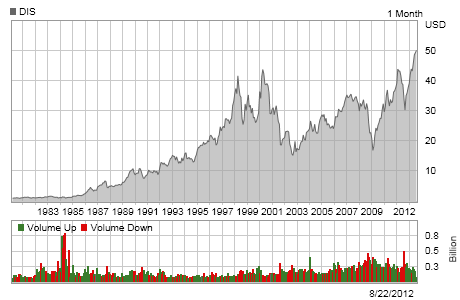
\includegraphics{DisneyChart.png}      %-- include image file named as "disneychart.png" 
   \caption{This is the figure's caption -- Disney stock chart}
    \label{fig:disneystock}
\end{figure}


Some notes on citing references.   When using APA format, the author-date method of citation is 
followed.   This means that the author's last name and the year of publication for the source should 
appear in the text, and a complete reference should appear in the reference list.

%
% Examples:
%     	Smith (1970) compared reaction times . . .
%     	In a recent study of reaction times (Smith, 1970), . . .   
%     	In 1970, Smith compared reaction times . . .
%	Smith, et al., (1970) compared reaction times . . .
%     	In a recent study of reaction times (Smith, et al., 1970), . . .  
%     	In 1970, Smith, et al., compared reaction times . . .
%

Here are some examples on how to do the referencing (note author's name and years are different
from commented examples).  For APA citation details, refer
to \url{http://www.ctan.org/tex-archive/biblio/bibtex/contrib/apacite/}. 

\begin{itemize}
 \item \citeA{kartch:2000:ERA} compared reaction times...
 \item In a recent study of reaction times \cite{kartch:2000:ERA}...
 \item In \citeyearNP{kartch:2000:ERA}, \citeauthor{kartch:2000:ERA} compared reaction times...
 \item \shortciteA{fedkiw:2001:VSO} compared reaction times... 
 \item In a recent study of reaction times \cite{fedkiw:2001:VSO}...
 \item In \citeyearNP{fedkiw:2001:VSO}, \shortciteauthor{fedkiw:2001:VSO}, compared reaction times...
\end{itemize}

The following are references from journal articles \cite{Park:2006:DSI, Pellacini:2005:LAH, 
sako:2001:SSB}.  Here's an MS thesis document \cite{yee:2000:SSA}, and this is from
PhD dissertation \cite{kartch:2000:ERA}. For a book, reference is given as 
\cite{parke:1996:CFA}.  Proceedings from a conference samples are \cite{Jobs95, fedkiw:2001:VSO,
levoy:2000:TDM}.  The sample bibliography file named \textbf{myreferences.bib} is from the
SIGGRAPH \LaTeX template.  You can use a text editor to view the contents of the bib file.  
It is your task to create your own bibliography file.  For those who downloaded papers from
ACM or IEEE sites, there is a BibTeX link that you can click; thereafter, you just simply need
to copy and paste the BibTeX entry into your own bibliography file.



The following shows how to include a program source code (or algorithm).  The verbatim environment,
as the name suggests, outputs text (including white spaces) as is...

\begin{verbatim}
               #include <stdio.h>
               main()
               {
                    printf("Hello world!\n");
               }
\end{verbatim}


\textcolor{red}{DO NOT FORGET to write the statement of the research problem here, i.e.,
before the Research Objectives.}



\section{Research Objectives}
\label{sec:researchobjectives}

\subsection{General Objective}
\label{sec:generalobjective}

This subsection states the over--all goal that must be achieved to answer the problem.
Address the following: Given your research challenge or opportunity, how do you intend 
to solve it? What is the output of your research?


\subsection{Specific Objectives}
\label{sec:specificobjectives}

\begin{enumerate}
	\item To develop a module to evaluate the affiliation of a set of users based on their social media posts.
	\item To implement a clustering algorithm that will identify communities based on the aforementioned affiliations
	\item To create a tool to visualize the communities in a user-friendly interface
\end{enumerate}

\section{Scope and Limitations of the Research}
\label{sec:scopelimitations}

This section discusses the boundaries (with respect to the objectives) of the research and the constraints within 
which the research will be developed.

\begin{comment}

%
% IPR acknowledgement: the sentences inside this comment are from Ethel Ong's slides on Scope and Limitations of the Research
%
Generally, one paragraph should be allotted for each of your research objectives.

Each paragraph contains a brief overview of the concept/theory and the purpose of doing the associated objective.

Each paragraph also includes a description of the scope/limitation of your study.

* Please refer to the slides for examples.

\end{comment}


\section{Significance of the Research}
\label{sec:significance}

This section explains why research must be done in this area.  It rationalizes the objective of the research with that of the stated problem. 
Avoid including sentences such as ``This research will be beneficial to the proponent/department/college'' as this is already an inherent
requirement of all BS and MS thesis projects.  Focus on the research's contribution to the Computer Science field.

The following are guide questions that may help your formulate the significance of your research. 


%
% IPR acknowledgement: the following list of items are from Ethel Ong's slides on Significance of the Research
%
\begin{itemize}
	\item  What is the relevance of your work to the computer science community? 

	\begin{itemize} 
	\item What will be your technical contributions, in terms of algorithms, or approaches, or new domain? 
	\item What is your value-added compared to existing systems? 
	\end{itemize}

	\item What will be your contributions to society in general? 
    \begin{itemize}
		\item This research will help certain stakeholders understand the common sentiments from social media users.
		\item This research will be useful in finding points of improvement in relevant institutions.
	\end{itemize}
\end{itemize}




               %-- includes LaTeX source file for Chapter 1: Research Description
                                  %-- your job: **EDIT THIS FILE** to indicate your own research description
\begin{comment}
%%%%%%%%%%%%%%%%%%%%%%%%%%%%%%%%%%%%%%%%%%%%%%%%%%%%%%%%%%%%%%%%%%%%%%%%%%%%%%%%%%%%%%%%%%%%%%%%%%%%%%
%
%   Filename    : chapter_2.tex 
%
%   Description : This file will contain your Review of Related Literature.
%                 
%%%%%%%%%%%%%%%%%%%%%%%%%%%%%%%%%%%%%%%%%%%%%%%%%%%%%%%%%%%%%%%%%%%%%%%%%%%%%%%%%%%%%%%%%%%%%%%%%%%%%%

\chapter{Review of Related Literature}
\label{sec:relatedlit}

This chapter discusses the features, capabilities, and limitations of existing research, algorithms, or software that are related or similar to the proposed research. This chapter is divided into three sections. The first section discusses algorithms for community detection. The second section discusses algorithms for sentiment analysis and other similarity parameters used for community detection. The third section discusses community evaluation metrics.

\begin{comment}
%
% IPR acknowledgement: the contents withis this comment are from Ethel Ong's slides on RRL.
%
Guide on Writing your RRL chapter

1. Identify the keywords with respect to your research
One keyword = One document section
Examples: 2.1 Story Generation Systems
2.2 Knowledge Representation

2.  Find references using these keywords

3.  For each of the references that you find,
Check: Is it relevant to your research?
Use their references to find more relevant works.

4. Identify a set of criteria for comparison.
It will serve as a guide to help you focus on what to look for

5. Write a summary focusing on -
What: A short description of the work
How: A summary of the approach it utilized
Findings: If applicable, provide the results
Why: Relevance to your work

6. At the end of each section,  show a Table of Comparison of the related works 
and your proposed project/system

\end{comment}

\section{Community Detection}

\citeA{Tang:2010} wrote a textbook on community detection. In the book, they sought to introduce characteristics of social media, review representative tasks of computing with social media, and illustrate associated challenges because with the emergence of social media websites, they felt it was an avenue to study human interaction and collaboration on an unparalleled scale. Multiple community detection approaches were discussed such as node-centric, network-centric, and hierarchy-centric. 

Node-centric algorithms involve the maximum clique detection problem which involves searching for a maximum complete subgraph of nodes in a network graph that are all adjacent to each other. The clique percolation method can find overlapping communities by finding cliques of size k, and then producing a clique graph, wherein two cliques are connected if they share k-1 nodes. Each connected element in this clique graph is then a community.

Network-centric algorithms involves vertex similarity, which is the similarity of the node’s social circles or how many common friends the two nodes have. This is what structural equivalence deals with. Two nodes $v_i$ and $v_j$ are structurally equivalent if $\forall v_k \in \{x \mid x \neq v_i \wedge x \neq v_j \}$ $e(v_i,v_k) \in E \iff e(v_j,v_k) \in E$, which is to say, $v_i$ and $v_j$ are connected to the exact same nodes. Nodes that are structurally equivalent belong to a community. 

Hierarchy-centric algorithms come in two forms: divisive and agglomerative. In divisive clustering, the entire set of nodes starts out in one set and each time, each set is divided into two until each community only has one member. The division is done by finding the node with the lowest edge betweenness and removing it, since that node is most likely the node connecting two communities. Agglomerative clustering starts with each node in their own community and communities are joined if they increase the overall modularity of the set of communities. Modularity is given by

\begin{equation}
Q = \frac{1}{2m} \sum_{l = 1}^{k} \sum_{i \in C_l, j \in C_l} (A_{ij} - \frac{d_i d_j}{2m})
\end{equation}

Where $m$ is the number of edges, $d_i$ is the degree of node $v_i$, $C_l$ being the $lth$ community, and $A_ij$ being the value in the adjacency matrix for node $v_i$ and $v_j$.

These algorithms may be considered in the final community detection phase of the proposed research \cite{Tang:2010}.

\citeA{Lim:2012:1} aimed to detect communities that share common interests on Twitter, based on linkages among followers of celebrities representing an interest category because they wish to help markets identify target groups with common interests. However, their approach differs from the typical  paradigm of ''identify communities then, for each, identify interests'', for they first identified interests they wish to extract communities from and from these interests, they then extracted the communities. 

Given a set of celebrities, C, celebrities being users with more than ten thousand followers, the algorithm first gets the common followers of all the celebrities in the set using the formula. 

\begin{equation}
P = \bigcap_{j \in C} (\bigcup_i link(i,c_j))
\end{equation}

Where $link(i,j)$ is given by

\begin{equation}
link(i,j) = \begin{cases}
\{i\} & \text{i follows j} \\
\emptyset & \text{i does not follow j}
\end{cases}
\end{equation}

Given this set of fans, P, they used the Infomap Algorithm and the Clique Percolation Method to detect communities in P. For each interest they wish to extract communities for, they chose the top 6 most popular celebrities based on follower count. Google and Wikipedia were used to identify which interests a celebrity represents. Afterwards, all users that follow the 6 celebrities were selected. They then selected 200,858 random users as a control group. Their algorithm produced more communities and larger communities than the control group, as well as more consistent communities, having a higher clustering coefficient. 

This paper provides an interesting alternative to detect communities by first specifying the interest of the community before detecting it, which may be used in the proposed research on top of the usual algorithms \cite{Lim:2012:1}.


\citeA{Zhang:2012} sought to identify communities in Twitter based on common interests. This is because Twitter has become very popular recently but little is known of it in the user level. This study would help in user recommendation and tweet recommendation as well as viral marketing to specific target groups. To identify the communities, they first compute specific feature similarities, then aggregate these features to compute for the final user similarity, and then they used classical clustering algorithms to detect the communities. To identify the communities, they first compute specific feature similarities, then aggregate these features to compute for the final user similarity, and then they used classical clustering algorithms to detect the communities.

The specific features they used were textual contents. Each data point was the entirety of a user’s tweets. Latent Dirichlet Allocation was used to identify latent topics from the user’s tweets. URL similarity was also detected, finding which users share similar links. Hashtag similarity was also analyzed. The social structure of users was also analyzed, which includes following similarity and retweeting similarity. 

In aggregating these similarities, the weighted sum of the previous similarities was computed to get the final similarity. Finally, k-means clustering was used to detect the communities based on their computed similarities. 

This paper presents a possible framework for detecting the communities. The proposed research may even use similar features, in addition to the Facebook specific features, to detect similarity. The k-means clustering algorithm will be one of the proposed algorithms for use in the proposed research \cite{Zhang:2012}.

\citeA{Deitrick:2013} sought to use sentiment classification to analyze communities in Twitter because harvesting information from these online social networks (OSN) would aid in the fields of politics and marketing. 

Their process is as follows: The follower network was represented as a weighted directed graph, each with initial weight of 1. To augment this, replies, mentions, retweets, hashtags, and sentiment classification of tweets were also harvested. These factors adjusted the weights in the graph. For community detection, the Infomap algorithm and Speaker-listener Label Propagation Algorithm(SLPA) were run. 

Generally, the network with updated weights produced communities with greater modularity. Of the two algorithms, the Infomap algorithm performed better. Recurring sentiment analysis was also helped by performing the aforementioned algorithms on the accounts that have already been placed in detected communities, which permits more in-depth analysis into the user’s sentiment since it could be analyzed within the context of the detected community.

This research provides a new way to represent the network, with their updated weights, as well as more possible algorithms to consider in detecting communities \cite{Deitrick:2013}.

\citeA{Cao:2015} proposed a visual analysis system, SocialHelix, because social media is a grand avenue for people to express their opinions and the researchers believed that an intuitive visualization that unfolds the process of sentiment divergence would have a far-reaching impact on multiple domains. 

They first identified the key domain problems of social divergence before employing a data abstraction design to convert the raw data into a form that captures all the key factors of the aforementioned domain problems. This abstracted data is then represented in a visualization based on a visual DNA metaphor. In identifying the key domain problems, it is determined when divergences start and end, how they evolve, who is involved, what roles do they play, and why does divergence occur. In the abstraction phase, the raw data is decomposed into temporal extent of social communities, topics or events, and user responses to these topics or events. In the visualization phase, the opposite sides of the helix represent the two sides of a divergence. The helix curves represents the changes in the communities’ sentiment. Nucleobase pairs represents events that connect the two communities. 

In implementation, the data was first filtered, removing unrelated posts and people. Statistical Linguistic Sentiment Analysis was used to determine the user’s sentiment. Finally, clustering was done using Hadoop, producing a cluster with 30 nodes. 

In the end, all test users were impressed by the visualization and agreed with the researchers’ model for the visualization. All test users felt that divergence identification was made easy due to the visualization. 

This research gives a sample visualization that can inspire the proponent’s own visualization, albeit the goal is not to model single divergences but an entire community. A possible tool, Hadoop, is also mentioned, which may be used to cluster the data \cite{Cao:2015}.

\section{Similarity Parameters}
This section outlines the basis/features/parameters used in detecting communities. It is divided into two subsections. The first subsection deals solely with sentiment analysis. The second subsection deals with other network and node parameters not related to sentiment analysis. 

\subsection{Sentiment Analysis}

\citeA{Zhang:2012} provided a formula to determine similarity in terms of text. 

\begin{equation}
sim_{text}(i,j) = \frac{1}{\sqrt{D_{js}(i,j)}}
\end{equation}

$D_{js}$ is the Jensen-Shannon Divergence between the two user’s topic probability distribution given by

\begin{equation}
D_{js}(i,j) = \frac{D_{kl}(UT_i \mid\mid M) + D_{kl}(UT_j \mid\mid M)}{2}
\end{equation}

Where $M = \frac{UT_i + UT_j}{2}$ and $D_{kl}(P \mid\mid Q) = \sum_{i \in topics} P(i) \log{\frac{P(i)}{Q(i)}}$ and $UT_i$ is the probability distribution of user i for all topics. $UT_i[t]$ is the probability distribution for user i on topic t.

This research provides a metric to determine the similarity of two users in terms of post content, which can be used in the proposed research \cite{Zhang:2012}.

\citeA{Deitrick:2013} used a subjective/objective and positive/negative Naive Bayes classifier. To do this, all tweets were converted to lowercase; hashtags, usernames, urls were replaced with twitterhashtag, twitterusername, and twitterurl respectively; the tweet text was tokenized; repeated punctuation was replaced with the + sign e.g. !!! -> !+; sentence punctuation was split into separate tokens; non-sentence punctuation was removed. Ten-fold cross validation was used in training the classifier. Weights in the graph mentioned in section 2.1 were then updated if two users posted something with a similar sentiment and similar hashtag. 

This research shows a clearly defined process in performing sentiment analysis, particularly the data cleaning step. This process could be adapted for the proposed research \cite{Deitrick:2013}.

\subsection{Other Parameters}

\citeA{Zhang:2012} provided a few formulas to determine similarity in terms of URL, hashtag, following, and retweeting similarity.

URL similarity is given by the same formula as text similarity in section 2.2.1, only using links instead of topics.

Hashtag similarity is given by 

\begin{equation}
sim_{hashtag}(i,j) = \sum_{k=1}^n (1 - \left|{\frac{N_{ik}}{\left|{H_i}\right|} - \frac{N_{jk}}{\left|{H_j}\right|}}\right|)\frac{N_{ik} + N_{jk}}{\left|{H_i}\right| + \left|{H_k}\right|}
\end{equation}

Where $N_{ik}$ is the number of times user $v_i$ used the hashtag $k$ while $H_i$ is the total hashtags used by $v_i$.

Following similarity is given by 

\begin{equation}
sim_{follow}(i,j) = \frac{c_{friend}}{\sqrt{\left|{Friend_i}\right|\left|{Friend_j}\right|}} + \frac{c_{follower}}{\sqrt{\left|{Follower_i}\right|\left|{Follower_j}\right|}}
\end{equation}

$\left|{Friend_i}\right|$ is the total number of users $v_i$ follows. $\left|{Follower_i}\right|$ is the total number of users that follow $v_i$. $c_{friend}$ represents the two users’ common friends. $c_{follower}$ represents the two users’ common followers.

Retweeting similarity is given by 

\begin{equation}
sim_{retweet}(i,j) = \frac{c_{retweet}}{\sqrt{\left|{R_i}\right|\left|{R_j}\right|}} + \frac{n_{ij} + n_{ji}}{\left|{R_i}\right|\left|{R_j}\right|}
\end{equation}

$R_i$ is the number of users whom $v_i$ retweet. $c_{retweet}$ is the number of users both $v_i$ and $v_j$ retweet. $n_{ij}$ is the number of times $v_i$ retweeted $v_j$ and $n_{ji}$ is the inverse case. 

The aggregate similarity is now given by

\begin{equation}
sim(i,j) = \gamma_t sim_{text} + \gamma_u sim_{url} + \gamma_h sim_{hashtag} + \gamma_f sim_{follow} + \gamma_r sim_{retweet}
\end{equation}

With $\gamma_{feature}$ determined in a process described in section 2.3.

This research gives formulas that can be used in the proposed research to measure similarity \cite{Zhang:2012}. 

\section{Community Evaluation Metrics}

\citeA{Zhang:2012} used the average number of mutual following links per user per community(FPUPC) to evaluate their communities. Based on this, appropriate weights for the aggregation were found by first performing their k-means clustering algorithm using only one feature similarity for each of the similarities and extracting the FPUPC. Afterwards, they gave each feature similarity a weight based on the following formula. 

\begin{equation}
w_{feature} = \frac{FPUPC_{feature}}{\sum_{f \in features} FPUPC_f}
\end{equation}

The number of clusters, k, used in the k-means clustering algorithm was also tweaked to get the maximum FPUPC. They concluded that they were successful in generating relatively accurate communities due to the incrementally increasing FPUPC after adjusting the weights.

This provides one possible evaluation metric for the proposed research, as well as a method to provide weights for the feature similarities that the proponents will eventually be using for community detection \cite{Zhang:2012}.
\begin{landscape}
	\begin{table}
		\centering
		\caption {Summary of Review of Related Literature}
		\begin{tabu}{| X[l] | X[l] | X[l] | X[l] | X[l] |}
			\hline
			Reference & Community Detection Algorithms & Sentiment Analysis Model & Other parameters & Community Evaluation \\
			\hline
			\cite{Tang:2010} & Clique percolation method, similarity detection, divisive and agglomerative clustering & & & \\
			\hline
			\cite{Lim:2012:1} & Topic driven community detection, Infomap method, Clique percolation method & & & \\
			\hline
			\cite{Zhang:2012} & k-means clustering & Similarity Formula for Text & Similarity Formula for URL, Hashtag, Follower, and Retweeting & FPUPC metric \\
			\hline
			\cite{Deitrick:2013} & Weighted directed graph, Infomap Algorithm, SLPA & Subjective/Objective, Positive/Negative Naive Bayes Classifier & replies, mentions, retweets, hashtags & \\
			\hline
			\cite{Cao:2015} & Data abstraction design, Hadoop tool & Temporal extent of posts, topics and events, user responses, Statistical Linguistic Sentiment Analysis & & \\
			\hline
		\end{tabu}
	\end{table}
\end{landscape}               %-- includes LaTeX source file for Chapter 2: Review of Related Literature
                                  %-- your job: **EDIT THIS FILE** to indicate your review of related literature 

%%%%%%%%%%%%%%%%%%%%%%%%%%%%%%%%%%%%%%%%%%%%%%%%%%%%%%%%%%%%%%%%%%%%%%%%%%%%%%%%%%%%%%%%%%%%%%%%%%%%%%
%
%   Filename    : chapter_3.tex 
%
%   Description : This file will contain your Research Methodology.
%                 
%%%%%%%%%%%%%%%%%%%%%%%%%%%%%%%%%%%%%%%%%%%%%%%%%%%%%%%%%%%%%%%%%%%%%%%%%%%%%%%%%%%%%%%%%%%%%%%%%%%%%%

\chapter{Research Methodology}
This chapter lists and discusses the specific steps and activities that will be performed by the proponent to accomplish the project. 
The discussion covers the activities from pre-proposal to Final Thesis Writing.  It also includes an initial discussion on the theoretical
framework to be followed.

\section{Research Activities}
Research activities include inquiry, survey, research, brainstorming, canvassing, consultation, review, interview, observe, experiment, design, 
test, document, etc.  The methodology also includes the following information:

\begin{itemize}
   \item who is responsible for the task
   \item the resource person to be contacted
   \item what will be done
   \item when and how long will the activity be done
   \item where will it be done
   \item why should be activity be done
\end{itemize}


\section{Calendar of Activities}

A Gantt chart showing the schedule of the activities should be included as a table. For example:

Table \ref{tab:timetableactivities} shows a Gantt chart of the activities.  Each bullet represents approximately
one week worth of activity.

%
%  the following commands will be used for filling up the bullets in the Gantt chart
%
\newcommand{\weekone}{\textbullet}
\newcommand{\weektwo}{\textbullet \textbullet}
\newcommand{\weekthree}{\textbullet \textbullet \textbullet}
\newcommand{\weekfour}{\textbullet \textbullet \textbullet \textbullet}

%
%  alternative to bullet is a star 
%
\begin{comment}
   \newcommand{\weekone}{$\star$}
   \newcommand{\weektwo}{$\star \star$}
   \newcommand{\weekthree}{$\star \star \star$}
   \newcommand{\weekfour}{$\star \star \star \star$ }
\end{comment}



\begin{table}[ht]   %t means place on top, replace with b if you want to place at the bottom
\centering
\caption{Timetable of Activities} \vspace{0.25em}
\begin{tabular}{|p{2in}|c|c|c|c|c|c|c|c|} \hline
\centering Activities (2009) & Jan   & Feb & Mar & Apr & May & Jun & Jul \\ \hline
Study on Prerequisite Knowledge      &   &  & ~~~\weektwo & \weekfour &  &  &  \\ \hline
Review of Existing Racing Strategies & ~~~\weektwo  & \weekfour & \weekfour & \weekfour &  &  &  \\ \hline
Identification of Best Features      &   &  &  & \weekfour & \weektwo~~~ &  &  \\ \hline
Development of Racing Strategies     &   &  &  & ~~~\weektwo & \weekfour & \weektwo~~~ &  \\ \hline
Simulation of Racing Strategies      &   &  &  & ~~~\weektwo & \weekfour & \weekthree~~ &  \\ \hline
Analysis and Interpretation of the Results &   &  &  &  & \weekfour & \weekfour & \weekone~~~~~ \\ \hline
Documentation & ~~~\weektwo  & \weekfour & \weekfour & \weekfour & \weekfour & \weekfour & \weektwo~~~ \\ \hline
\end{tabular}
\label{tab:timetableactivities}
\end{table}

               %-- includes LaTeX source file for Chapter 3: Research Methodology
                                  %-- your job: **EDIT THIS FILE** to indicate your research methodology

\appendix                         %-- used to specify appendices
%%%%%%%%%%%%%%%%%%%%%%%%%%%%%%%%%%%%%%%%%%%%%%%%%%%%%%%%%%%%%%%%%%%%%%%%%%%%%%%%%%%%%%%%%%%%%%%%%%%%%%
%
%   Filename    : appendix_A.tex 
%
%   Description : This file is one of the appendices. 
%                 
%%%%%%%%%%%%%%%%%%%%%%%%%%%%%%%%%%%%%%%%%%%%%%%%%%%%%%%%%%%%%%%%%%%%%%%%%%%%%%%%%%%%%%%%%%%%%%%%%%%%%%

\chapter{Diagrams and Other Documentation Tools}
\label{sec:appendixa}


This appendix may consist of proposed architectural design, algorithms, scientific formula for 
MSCS and Data Flow Diagrams, Fishbone for MSIT.


              %-- includes LaTeX source file for Appendix A
                                                 %-- your job: **CREATE/EDIT** your own source file for the appendices
%%%%%%%%%%%%%%%%%%%%%%%%%%%%%%%%%%%%%%%%%%%%%%%%%%%%%%%%%%%%%%%%%%%%%%%%%%%%%%%%%%%%%%%%%%%%%%%%%%%%%%
%
%   Filename    : appendix_B.tex 
%
%   Description : This file will contain one of your appendices.
%                 
%%%%%%%%%%%%%%%%%%%%%%%%%%%%%%%%%%%%%%%%%%%%%%%%%%%%%%%%%%%%%%%%%%%%%%%%%%%%%%%%%%%%%%%%%%%%%%%%%%%%%%

\chapter{Theoretical and/or Conceptual Framework}
\label{sec:appendixb}

Discusses the basic framework/foundation the thesis is based on. This section is normally referred to when discussing Scope and Limitations,
and Research Methodology



%%%%%%%%%%%%%%%%%%%%%%%%%%%%%%%%%%%%%%%%%%%%%%%%%%%%%%%%%%%%%%%%%%%%%%%%%%%%%%%%%%%%%%%%%%%%%%%%%%%%%%
%
%   Filename    : appendix_C.tex
%
%   Description : This file will contain information about your Resource Persons
%                 
%%%%%%%%%%%%%%%%%%%%%%%%%%%%%%%%%%%%%%%%%%%%%%%%%%%%%%%%%%%%%%%%%%%%%%%%%%%%%%%%%%%%%%%%%%%%%%%%%%%%%%

\chapter{Resource Persons}
\label{sec:appendixc}

%
%  Indicate your resource persons here:
%
%	<full name and title, e.g., Dr. Juan de la Cruz>
%	<profession, e.g., faculty>
%	<department, e.g., College of Computer Studies>
%	<name of institution, e.g., De La Salle University>
%	<e-mail address>
%
%

%
%  the following shows 3 examples, replace entries with your own
%
\newcommand{\resperson}[4]{\textbf{#1} \\ #2 \\ #3 \\ \url{#4}\vspace{0.5em}\\}

\resperson{Ms. Charibeth Cheng}{Adviser}{College of Computer Studies\\De La Salle University-Manila}{chari.cheng@delasalle.ph}
%\resperson{Mr. Firstname2 Lastname2}{Role2}{Affiliation2}{emailaddr2@domain.com}
%\resperson{Ms. Firstname3 Lastname3}{Role3}{Affiliation3}{emailaddr3@domain.net}




%\bibliographystyle{apacite}       %-- specified APA style for bibliograpy
                                  %-- more details about APA style citation can be found in www.ctan.org/tex-archive/biblio/bibtex/contrib/apacite/

                                  %-- bibliographic entries are handled via bibtex; refer to www.bibtex.org for more details
\end{comment}

\bibliography{myreferences}       %-- the file "myreferences.bib" is a sample bibliography (bib) from SIGGRAPH 
                                  %-- your job: **CREATE/EDIT** your own bibliography file  

\end{document}

